
%-----------------------------  README  ------------------------------------------
% THESIS TEMPLATE FILE - compatible with University of Leeds guidelines, and designed
% for use when submitting an alternative format thesis / thesis by publication.
% Key point is that by using biber instead of bibtex, bibliographies for each publication
% can be created from a single .bib file.
%
% Instructions:
%   - To compile:
%     pdflatex alt_format_thesis.tex
%     biber alt_format_thesis                   % NOTE NO EXTENSION FOR BIBER!
%     pdflatex alt_format_thesis.tex
%
% Installing / getting it to compile:
%    When used with TexLive on Ubuntu 18.04, some other packages and biber are needed:
%    e.g. in a terminal:
%     sudo apt install texlive-bibtex-extra                                            % Usually missing if breakcites.sty can't be found
%     sudo apt install biber                                                           % used instead of biblatex as it supports refsections (which allows a bibliography in each chapter from a single .bib file)

%    Others that may be needed:
%      sudo apt-get install texlive-fonts-extra
%
%     Errors from missing .sty files are usually to do with missing packages.
%
% Latexdiff:
%    Great for tracking changes.  A nice guide to what can be a tricky install is here:
%    http://www.deanbodenham.com/learn/troubleshooting-latexdiff.html


% History
%     M.C.   Garthwaite 30/09/2011
%     D.P.S. Bekaert 	23/02/2016  Adapt for thesis by publication
%     M.E. 	 Gaddes		13/03/2019	Adapt to handle references from a single .bib file
%     M.E.   Gaddes   05/06/2020  Create minimum working template

%-----------------------------------------------------------------------




\documentclass[titlepage,twoside,onecolumn,a4paper,11pt]{report}

\edef\restoreparindent{\parindent=\the\parindent\relax}
\usepackage{parskip}
\restoreparindent

\usepackage{float}
\usepackage{fancyhdr} 												% for making headers and footers
\usepackage{appendix} 												% sets up the appendix environment
\usepackage{graphicx} 												% Needed to display graphics
\usepackage{geometry}                   % Allows definition of text/page measurements
\usepackage{setspace} 												% \singlespacing , \onehalfspacing , and  \doublespacing
\usepackage{url} 													% line-breaks for long URLs, DOIs, etc
\usepackage{amsmath} % AMS mathematics
\usepackage{amssymb} % Defines names of maths symbols in amsfonts
\usepackage{a4} % for A4 paper size. Not needed if defined in \documentclass ?
\usepackage{enumitem} % useful for customising lists
\usepackage[small,bf]{caption} % Sets the style of the captions for figure/table. here the text
\usepackage[left,mathlines]{lineno}  % Places line numebrs in margin
\usepackage[nottoc,notbib]{tocbibind}
\usepackage[pdftex,pdfpagelabels,breaklinks=true]{hyperref}  % Creates hyper links N.B. pdf option and index option [pdftex,hyperindex,backref,pdfpagelabels]
\usepackage[all]{hypcap} % Hyperlinks go to all of figure rather than just caption. Problem if figure does not have a caption - Conflicts with {fltpage}
%\usepackage{doi}  % Need to download sty file. Add doi links N.B. must go after hyperref. Also it won't work with doi's with < >. For % put \%. doi links are only compatible with certain bib style files
\usepackage[normal]{subfigure} % allows multiple floats within one figure environment with a caption for each in addition to main caption
\usepackage{breakcites}
%\usepackage{breakurl}
\usepackage{makeidx} % Make Index
\makeindex

\usepackage{multirow}


%%%%%%%%%%%%%%%%%%%% Bibliography stuff. Argh!!!!
%\usepackage[backend=biber, style=apa, natbib=true, citestyle=authoryear, uniquename=false, maxcitenames=1]{biblatex}		          %
\usepackage[backend=biber,
            natbib=true,                                % using natbib allows the use of citet and citep, so you can copy from JGR file
            citestyle=authoryear,                       %
            bibstyle=authoryear,                        % no number of bibliography
            maxcitenames=2,                             % switch to firsname + et al if more than 2
            maxbibnames=99,                             % don't truncate authors to et al in bibliography
            uniquename=false,                           % control inititals and get correct number of authors (no name1, name2, et al)
            uniquelist=false,                            % ditto
            ]{biblatex}
%\addbibresource{library_2019_05_01.bib}                     % include extension for biber
%\addbibresource{library_2019_05_13.bib}                     % include extension for biber
%\addbibresource{library_2019_06_16.bib}                     % include extension for biber
\addbibresource{library.bib}                     % include extension for biber
%%%%%%%%%%%%%%%%%%%% End Bibliography stuff.



%%%% Pdf name etc setup
\hypersetup{
    plainpages=false,                   % Resets counter in main matter (Problems of links to early pages)
    bookmarks=true,                     % show bookmarks bar?
    unicode=false,                      % non-Latin characters in Acrobat\u2019s bookmarks
    pdftoolbar=true,                    % show Acrobat\u2019s toolbar?
    pdfmenubar=true,                    % show Acrobat\u2019s menu?
    pdffitwindow=true,                  % page fit to window when opened
    pdfstartview={FitV},
    pdftitle={Automatic Detection of Volcanic Unrest Using Synthetic Aperture Radar},    % title
    pdfauthor={Matthew Edward Gaddes},     % author
    pdfcreator={School of Earth and Environment, University of Leeds},
    pdfsubject={PhD Thesis, School of Earth and Environment, University of Leeds},   % subject of the document
    pdfkeywords={},
    pdfdisplaydoctitle=true,
    % SET up LINKS
    colorlinks=true,% false: boxed links; true: colored links
    citecolor=black,% color of links to bibliography
    filecolor=black,% color of file links
    linkcolor=black,% color of internal links
    urlcolor=black% color of external links
}


%\DeclareUnicodeCharacter{0301}{*************************************}          # good for hunting for unicode errors.


%%%% Page setup
\pagestyle{fancy} % 'fancy' will place header and footers. 'plain' will not
\renewcommand{\chaptermark}[1]{\markboth{\chaptername\ \thechapter:\ #1}{}} %% sets format of Chapter mark (left pages)
\renewcommand{\sectionmark}[1]{\markright{\S\thesection\ #1}} %% sets format of section mark (right pages)
\renewcommand{\headrulewidth}{0.5pt} %%sets thickness of header rule
\renewcommand{\footrulewidth}{0pt}  %%sets thickness of footer rule
\fancyhead[RO,LE]{\thepage} 							% options R - Right-hand side L - Left-hand side O - odd page E - even page
% \fancyhead[RE]{\nouppercase\leftmark}
% \fancyhead[LO]{\nouppercase\rightmark}
\fancyfoot{}
%\setlength\headheight{13.6pt}					% if paper titles stay on one page in the headers
\setlength\headheight{26.0pt}					% if paper titles go onto two pages in the headers
\fancyhfoffset[EL,OR]{0mm}
\onehalfspacing							 % alternative \doublespacing. both acceptable for Leeds submissions
%\geometry{a4paper,twoside,inner=40mm,outer=25mm,top=30mm,bottom=35mm}		% Definition of page measurements compatible with University of Leeds margin requirements (40mm x 20mm x 20mm x 20mm).
\geometry{a4paper,inner=40mm,outer=25mm,top=30mm,bottom=35mm}				% Larger margin for binding side
%%%% End page setup

%%%%%%%%%%%%%%%%%%%%%%%%%%%%%%%%%%%%%%%%%%%%%%%%%%%%%%%%%%%%%%%%%%%%%%%%%%%%%%%%%%%%%%%%%%%% End Preamble %%%%%%%%%%%%%%%%%%%%%%%%%%%%%%%%%%%%%%%%%%%%%%%%%%%%%%%%%%%%%%%%%%%%%%%%%%%%%%%%%%%%%%%%%%%%
\begin{document}
\pagenumbering{roman} % Start roman numbering, to be used up until introduction.

\makeatletter
\def\cleardoublepage{\clearpage\if@twoside \ifodd\c@page\else%
\hbox{}%
\thispagestyle{empty}
\newpage%
\if@twocolumn\hbox{}\newpage\fi\fi\fi}
\makeatother

%%%%%%%%%%%%%%%%%%%%%%%%%%%% Title Page %%%%%%%%%%%%%%%%%%%%%%%%%%%%
\title{
\Huge{\textbf{My First Thesis}}\\[2cm]
\Large{{\bf First Second Surname}} \\[4cm]
\large{Submitted in accordance with the requirements for the degree of\\
Doctor of Philosophy} \\[2cm]
\large{The University of Leeds}\\
\large{School of Earth and Environment}\\ [2cm]
\large{May 2019} }
\author{} \date{}
\pdfbookmark[0]{Title page}{Title page} % Sets a PDF bookmark for the title page
\maketitle
\cleardoublepage

%%%%%%%%%%%%%%%%%%%%%%%%%%%% Declaration %%%%%%%%%%%%%%%%%%%%%%%%%%%%
% \fancyhead[RE,LO]{Declaration}						% text, right edge of even pages, left edge of odd
% \fancyhead[RO,LE]{\thepage}							% page number, right edge of odd pages, left of even
The candidate confirms that the work submitted is their own, except where work which has formed part of jointly authored publications has been included. The contribution of the candidate and the other authors to this work has been explicitly indicated below. The candidate confirms that appropriate credit has been given within the thesis where reference has been made to the work of others.\\

The work in Chapter \ref{ch:publication1} of the thesis has appeared in publication as follows:\\
Publication 1 citation.

Author 1 did...., Author 2 did...., author 3 did.... .
\vspace{5mm}

The work in Chapter \ref{ch:publication2} of the thesis has been accepted for publication pending minor revisions under the following title:\\
Paper 2 citation.

Author 1 did...., Author 2 did...., author 3 did.... .
\vspace{5mm}

The work in Chapter \ref{ch:publication3} of the thesis is a manuscript about to be submitted under the following title:\\
Publication 3 title.

Author 1 did...., Author 2 did...., author 3 did.... .
\vspace{5mm}

This copy has been supplied on the understanding that it is copyright material and that no quotation from the thesis may be published without proper acknowledgement\\

Copyright \copyright\; 2019 The University of Leeds and First Second Surname\\
The right of First Second Surname to be identified as Author of this work has been asserted by him in accordance with the Copyright, Designs and Patents Act 1988.
\cleardoublepage




%%%%%%%%%%%%%%%%%%%%%%%%%%%% Acknowledgments %%%%%%%%%%%%%%%%%%%%%%%%%%%%
\chapter*{Acknowledgements}
\fancyhead[RE,LO]{Acknowledgements}
\fancyhead[RO,LE]{\thepage}

Lorem ipsum dolor sit amet, consectetur adipiscing elit. Donec quis nibh et mi fermentum luctus. Suspendisse semper urna commodo, ultrices ligula a, mattis orci. Lorem ipsum dolor sit amet, consectetur adipiscing elit. Fusce pellentesque mauris sed blandit pulvinar. Cras magna tellus, finibus eget pretium at, ultricies at nulla. Phasellus eleifend vehicula odio eget porta. Nam venenatis aliquam gravida. Nam pretium dapibus est nec gravida.

Suspendisse lectus lectus, molestie nec velit vitae, pharetra venenatis metus. Mauris pellentesque consectetur euismod. Pellentesque congue aliquam eleifend. In hac habitasse platea dictumst. Donec eu leo vulputate, consequat lectus hendrerit, tempor diam. Donec consequat est augue, a convallis tortor mattis et. Ut in fermentum ipsum. Nulla orci lacus, egestas a accumsan vel, vehicula sit amet enim. Quisque eget ipsum nec felis euismod pretium id vitae orci. Donec non nulla odio. Nullam vel lacinia tortor, ac imperdiet quam.

Praesent quis purus leo. Phasellus non neque fringilla, accumsan odio in, faucibus massa. Curabitur vel dignissim turpis. Vestibulum ante ipsum primis in faucibus orci luctus et ultrices posuere cubilia curae; Etiam eleifend fermentum dolor sit amet efficitur. Cras semper quam eget nisl accumsan pulvinar. Duis quis velit neque.




\cleardoublepage

%%%%%%%%%%%%%%%%%%%%%%%%%%%% Abstract %%%%%%%%%%%%%%%%%%%%%%%%%%%%
\chapter*{Abstract}
\fancyhead[RE,LO]{Abstract}
\fancyhead[RO,LE]{\thepage}

Integer feugiat sapien nisl, in pellentesque quam porttitor in. Suspendisse tincidunt, nisi ut elementum eleifend, ex nibh tempus nisl, vel sagittis ligula urna sed diam. Quisque ac ipsum est. Proin quis ultricies nisi. Praesent pretium placerat neque vitae rhoncus. In hac habitasse platea dictumst. Sed consequat sed orci eget vehicula. Nam cursus molestie magna, vitae semper est rhoncus sed.

Integer finibus vel nisi a dictum. Aenean arcu nisl, vulputate a metus nec, volutpat convallis eros. Donec suscipit vel diam at tincidunt. Sed viverra risus non tincidunt pharetra. Pellentesque rhoncus placerat aliquam. Cras aliquet at nibh in ultrices. Nulla placerat lorem vitae dapibus convallis. Aliquam erat volutpat.

Etiam vestibulum metus turpis, eget accumsan lacus luctus sed. Sed pellentesque tempor nisi sit amet vestibulum. Pellentesque et massa turpis. Nulla consequat in est vel venenatis. Nullam commodo dolor vel elit pellentesque gravida. Integer commodo sagittis sapien, cursus ornare augue. Nunc interdum metus eu accumsan rhoncus. Donec vitae feugiat turpis. In nec iaculis diam.

Vestibulum vulputate magna in nibh volutpat suscipit. Phasellus venenatis magna metus, eu tristique eros rhoncus in. Nulla suscipit nisl justo, eu vulputate velit euismod ut. Donec vitae ipsum a ex dictum suscipit at et neque. Sed ut varius odio. Fusce non mauris dignissim, tincidunt metus finibus, commodo lacus. Maecenas id iaculis neque, eu elementum neque. Nulla nec lectus in augue molestie fringilla. Integer a odio sed urna dapibus consectetur.

Pellentesque in orci consequat leo suscipit tristique vel ut mi. Orci varius natoque penatibus et magnis dis parturient montes, nascetur ridiculus mus. Suspendisse sit amet gravida purus. Aliquam dapibus vulputate sollicitudin. Vivamus cursus leo ac dolor vestibulum pulvinar quis sit amet lorem. Phasellus egestas lacus eu condimentum vulputate. Nam sed mi at ante blandit tincidunt. Maecenas id semper orci. Phasellus eget sem aliquet erat auctor convallis. Curabitur nec augue eu tellus pulvinar pulvinar. Curabitur non erat vitae lorem lobortis scelerisque. Nam ultricies nulla vitae ex commodo elementum at id metus. Integer non sem sodales, congue neque id, dictum orci. In efficitur eros in dui suscipit ullamcorper. Vivamus suscipit eleifend elit ac bibendum. In sit amet sodales massa, id consequat magna.


\cleardoublepage



%%%%%%%%%%%%%%%%%%%%%%%%%%%% Contents page %%%%%%%%%%%%%%%%%%%%%%%%%%%%
\pdfbookmark[0]{Contents}{Contents}
\fancyhead[RE,LO]{Contents}
\fancyhead[RO,LE]{\thepage}
\tableofcontents
\cleardoublepage

%%%%%%%%%%%%%%%%%%%%%%%%%%%% Lis of figures %%%%%%%%%%%%%%%%%%%%%%%%%%%%
\fancyhead[RE,LO]{List of Figures}
\fancyhead[RO,LE]{\thepage}
\listoffigures
\cleardoublepage

%%%%%%%%%%%%%%%%%%%%%%%%%%%% Manual Nomenclature %%%%%%%%%%%%%%%%%%%%%%%%%%%%
% this is a fudge that doesn't use the nomencl package, but it's simple and easy to use
\chapter*{Nomenclature}
\fancyhead[RE,LO]{Nomenclature}
\fancyhead[RO,LE]{\thepage}

\textbf{List of acronyms}\\ \\
\begin{minipage}{0.2\linewidth}
	BSS\\
    CNN\\
    DEM\\
    ESA\\
    GNSS\\
    GPS\\
    ICA\\
    InSAR\\
    NN\\
    NMF\\
    PCA\\
    PDF\\
    SAR\\
    SRTM\\
    SVM\\


\end{minipage}
\begin{minipage}{0.6\linewidth}
    Blind Signal Separation\\
    Convolutional Neural Network\\
    Digital Elevation Model\\
    European Space Agency\\
    Global Navigation Satellite System\\
    Global Positioning System\\
    Independent component analysis\\
    Interferometric synthetic aperture RaDAR\\
    Neural Network\\
    Non-negative matrix factorisation\\
    Principal component analysis\\
    Probability density function\\
    Synthetic aperture RaDAR\\
    Shuttle RaDAR Topography Mission\\
    Support vector machines\\


\end{minipage}

\noindent
\textbf{List of symbols}\\ \\
\begin{minipage}{0.2\linewidth}
	$\textbf{W}$\\
	$\textbf{A}$\\
	$\textbf{S}$\\
	$\textbf{X}$\\


\end{minipage}
\begin{minipage}{0.6\linewidth}
    Unmixing matrix\\
    Mixing matrix\\
    Sources (as row vectors)\\
    Mixtures (as row vectors)\\

\end{minipage}
\cleardoublepage
\fancyhead[RE]{\leftmark}		% Return Headers to Normal
\fancyhead[LO]{\rightmark}




\pagenumbering{arabic}           % Switch to normal numbers, also resets counter
\onehalfspacing
\begin{refsection}
\chapter[Introduction]{Introduction}
\label{ch:introduction}

Aliquam erat volutpat. Nam iaculis euismod urna. Ut neque lacus, condimentum dignissim sem ac, elementum lacinia quam. Vestibulum a dictum justo, non dignissim ipsum. Donec massa nunc, suscipit in tincidunt a, efficitur ac eros. Nulla nec eros elementum, feugiat velit vitae, hendrerit lacus. Curabitur tortor leo, cursus vel ante hendrerit, vulputate fermentum nisl. Praesent fringilla vitae ante at molestie. Nullam lacinia nibh eget rhoncus tristique.

A citation, either \citep{Massonet1998} or \citet{Massonet1998}

\begin{equation}
	Binary \ output =
  \begin{cases}
    1 & \text{if $\textbf{w}.\textbf{x}  > threshold$}\\
    0 & \text{if $\textbf{w}.\textbf{x} \leq threshold$}\\
  \end{cases}
\end{equation}


\section{A section}
\label{sec:volcano_monitoring_and_insar}


\begin{figure}[tbp]
	\centering
	\includegraphics[width=1\textwidth]{./front_material_figures/figure_3_sn_gps.png}
	\caption[Short Caption]{Long caption}
	\label{fig:population_volcanoes}
\end{figure}





\section{Aims and Objectives}
\label{sec:aims}
Mauris venenatis vitae tellus pharetra luctus. Donec egestas, neque at faucibus tincidunt, lorem ex accumsan nibh, sed lobortis magna leo ac lorem. Fusce luctus nibh et eros malesuada volutpat. Donec gravida ultrices ornare. Fusce maximus magna tortor, at tristique lectus mollis nec. Proin hendrerit rutrum tortor, eget varius velit ornare ut. Vestibulum hendrerit neque non venenatis tristique. Cras id ullamcorper tortor.

The objectives of this thesis are:

\begin{enumerate}
	\item{Objective 1}
	\item{Objective 2}
	\item{Objective }
\end{enumerate}




\section{Thesis outline}
\label{sec:outline}
The subsequent chapters in this thesis are organised as follows:

\begin{itemize}
  \item Chapter \ref{ch:publication1} blah blah.

  \item Chapter \ref{ch:publication2} more blah.

  \item Chapter \ref{ch:publication3} blah 3.


  \item Chapter \ref{ch:back_material} discusses the work contained within the preceding chapters in relation to the goal of Blah.
\end{itemize}



\printbibliography[heading=subbibliography]
\end{refsection}
\cleardoublepage

\cleardoublepage % dump remaining floats before end of chapter and ensure the next chapter starts on odd (right-hand) side
\fancyhead[RE]{\leftmark}
\fancyhead[LO]{\rightmark}


\onehalfspacing
\chapter[Publication 1 title]{Publication 1 title}
\label{ch:publication1}
\begin{center}
 \large{\textbf{F. surname}$^{\text{1}}$, A. Supervisor$^{\text{1}}$, and B. Supervisor$^{\text{2,3}}$  }  \\
\end{center}
\begin{center}
\textit{
$^{\text{1}}$ COMET, School of Earth and Environment, University of Leeds, United Kingdom\\
$^{\text{2}}$ Formerly, COMET, School of Earth and Environment, University of Leeds, United Kingdom\\
$^{\text{3}}$ Now at Jet Propulsion Laboratory, California Institute of Technology, Pasadena, CA, USA\\
}
\end{center}

\newpage
Key points:
\begin{itemize}
\item Some journals like key points.
\item Two.
\item Three.
\end{itemize}



\begin{refsection}
\section*{Abstract}
Aliquam erat volutpat. Nam iaculis euismod urna. Ut neque lacus, condimentum dignissim sem ac, elementum lacinia quam. Vestibulum a dictum justo, non dignissim ipsum. Donec massa nunc, suscipit in tincidunt a, efficitur ac eros. Nulla nec eros elementum, feugiat velit vitae, hendrerit lacus. Curabitur tortor leo, cursus vel ante hendrerit, vulputate fermentum nisl. Praesent fringilla vitae ante at molestie. Nullam lacinia nibh eget rhoncus tristique.



\section{Introduction} %%%%%%%%%%%%%%%%%%%%%%%%%%%%%%%%%%%%%%%%%%%%%%%%%%%%%%%%%%%%%%%%%%%%%%%%%%%%%%%%%%%%%%%%
\label{sec:intro}

\begin{figure}[tbp]
	\centering
	\includegraphics[width=1\textwidth]{./publication1_figures/figure_4_sn_ifgs.png}
	\caption[Short Caption]{Long caption}
	\label{fig:label2}
\end{figure}



A new citation: \citep{Bernard1997}


%% Biliogrpahy
% \newpage
% \baselineskip=11pt

\printbibliography[heading=subbibliography]
\end{refsection}

\cleardoublepage % dump remaining floats before end of chapter and ensure the next chapter starts on odd (right-hand) side
\fancyhead[RE]{\leftmark}
\fancyhead[LO]{\rightmark}


\include{publication2}
\cleardoublepage % dump remaining floats before end of chapter and ensure the next chapter starts on odd (right-hand) side
\fancyhead[RE]{\leftmark}
\fancyhead[LO]{\rightmark}


\onehalfspacing
\chapter[Publication 3 title]{Publication 3 title}
\label{ch:publication3}
\begin{center}
 \large{\textbf{F. surname}$^{\text{1}}$, A. Supervisor$^{\text{1}}$, and B. Supervisor$^{\text{2,3}}$}  \\
\end{center}
\begin{center}
\textit{
$^{\text{1}}$ COMET, School of Earth and Environment, University of Leeds, United Kingdom\\
$^{\text{2}}$ Formerly, COMET, School of Earth and Environment, University of Leeds, United Kingdom\\
$^{\text{3}}$ Now at Jet Propulsion Laboratory, California Institute of Technology, Pasadena, CA, USA\\
}
\end{center}

\newpage
Key points:
\begin{itemize}
\item Some journals like key points.
\item Two.
\item Three.
\end{itemize}



\begin{refsection}
\section*{Abstract}
Aliquam erat volutpat. Nam iaculis euismod urna. Ut neque lacus, condimentum dignissim sem ac, elementum lacinia quam. Vestibulum a dictum justo, non dignissim ipsum. Donec massa nunc, suscipit in tincidunt a, efficitur ac eros. Nulla nec eros elementum, feugiat velit vitae, hendrerit lacus. Curabitur tortor leo, cursus vel ante hendrerit, vulputate fermentum nisl. Praesent fringilla vitae ante at molestie. Nullam lacinia nibh eget rhoncus tristique.



\section{Introduction} %%%%%%%%%%%%%%%%%%%%%%%%%%%%%%%%%%%%%%%%%%%%%%%%%%%%%%%%%%%%%%%%%%%%%%%%%%%%%%%%%%%%%%%%
\label{sec:intro}

\begin{figure}[tbp]
	\centering
	\includegraphics[width=1\textwidth]{./publication3_figures/figure_11_activation_funcs.png}
	\caption[Short Caption]{Long caption}
	\label{fig:label2}
\end{figure}



A new citation: \citep{Bernard1997}
More citations: \citep{Hyvarinen1997}
And another: \citep{Mogi1958}

%% Biliogrpahy
% \newpage
% \baselineskip=11pt

\printbibliography[heading=subbibliography]
\end{refsection}

\cleardoublepage % dump remaining floats before end of chapter and ensure the next chapter starts on odd (right-hand) side
\fancyhead[RE]{\leftmark}
\fancyhead[LO]{\rightmark}


% InSAR thesis back material lengths
% Karsten - 5 pages
% Ruth Amey - 7 pages
% David - 12 pages
% George - 18 pages


\onehalfspacing
\begin{refsection}
\chapter[Discussion and Conclusions]{Discussion and Conclusions}
\label{ch:back_material}

Phasellus eget varius mauris. Integer faucibus pharetra enim posuere aliquet. Class aptent taciti sociosqu ad litora torquent per conubia nostra, per inceptos himenaeos. Pellentesque molestie, nisl id feugiat vehicula, neque nunc placerat ipsum, ut vehicula elit massa dictum orci. Morbi et ullamcorper felis. Fusce pretium ipsum eu sem tempus suscipit. Nullam sodales accumsan ligula, quis placerat urna laoreet id. Pellentesque porttitor et ligula vitae molestie. Class aptent taciti sociosqu ad litora torquent per conubia nostra, per inceptos himenaeos. Etiam tempor nibh quam, sit amet congue sapien suscipit at. Suspendisse in lorem leo. Pellentesque tempus at eros id consequat.

In this thesis, my objective was to develop an algorithm to detect signs of deformation-generating volcanic unrest in a time series of interferograms.  In Chapter \ref{ch:introduction} I divided this objective into four smaller aims, which I revisit in Section \ref{sec:disc_project_aims}.  In Section \ref{sec:disc_future_work} I discuss the opportunities for further work on this topic, and in Section \ref{sec:disc_conclusions} I present my concluding remarks.

Refs should still work:
A new citation: \citep{Bernard1997}
More citations: \citep{Hyvarinen1997}
And another: \citep{Mogi1958}



\section{Project aims and key findings}
\label{sec:disc_project_aims}


	\subsection{Further Remarks}
	\label{subsec:further_remarks}


	\subsection{Key Findings}
	\label{subsec:disc_key_findings}

	Some findings

	\begin{enumerate}
		\item{some stuff }
	\end{enumerate}




\section{Future work}
\label{sec:disc_future_work}


\begin{figure}[]
	\centering
	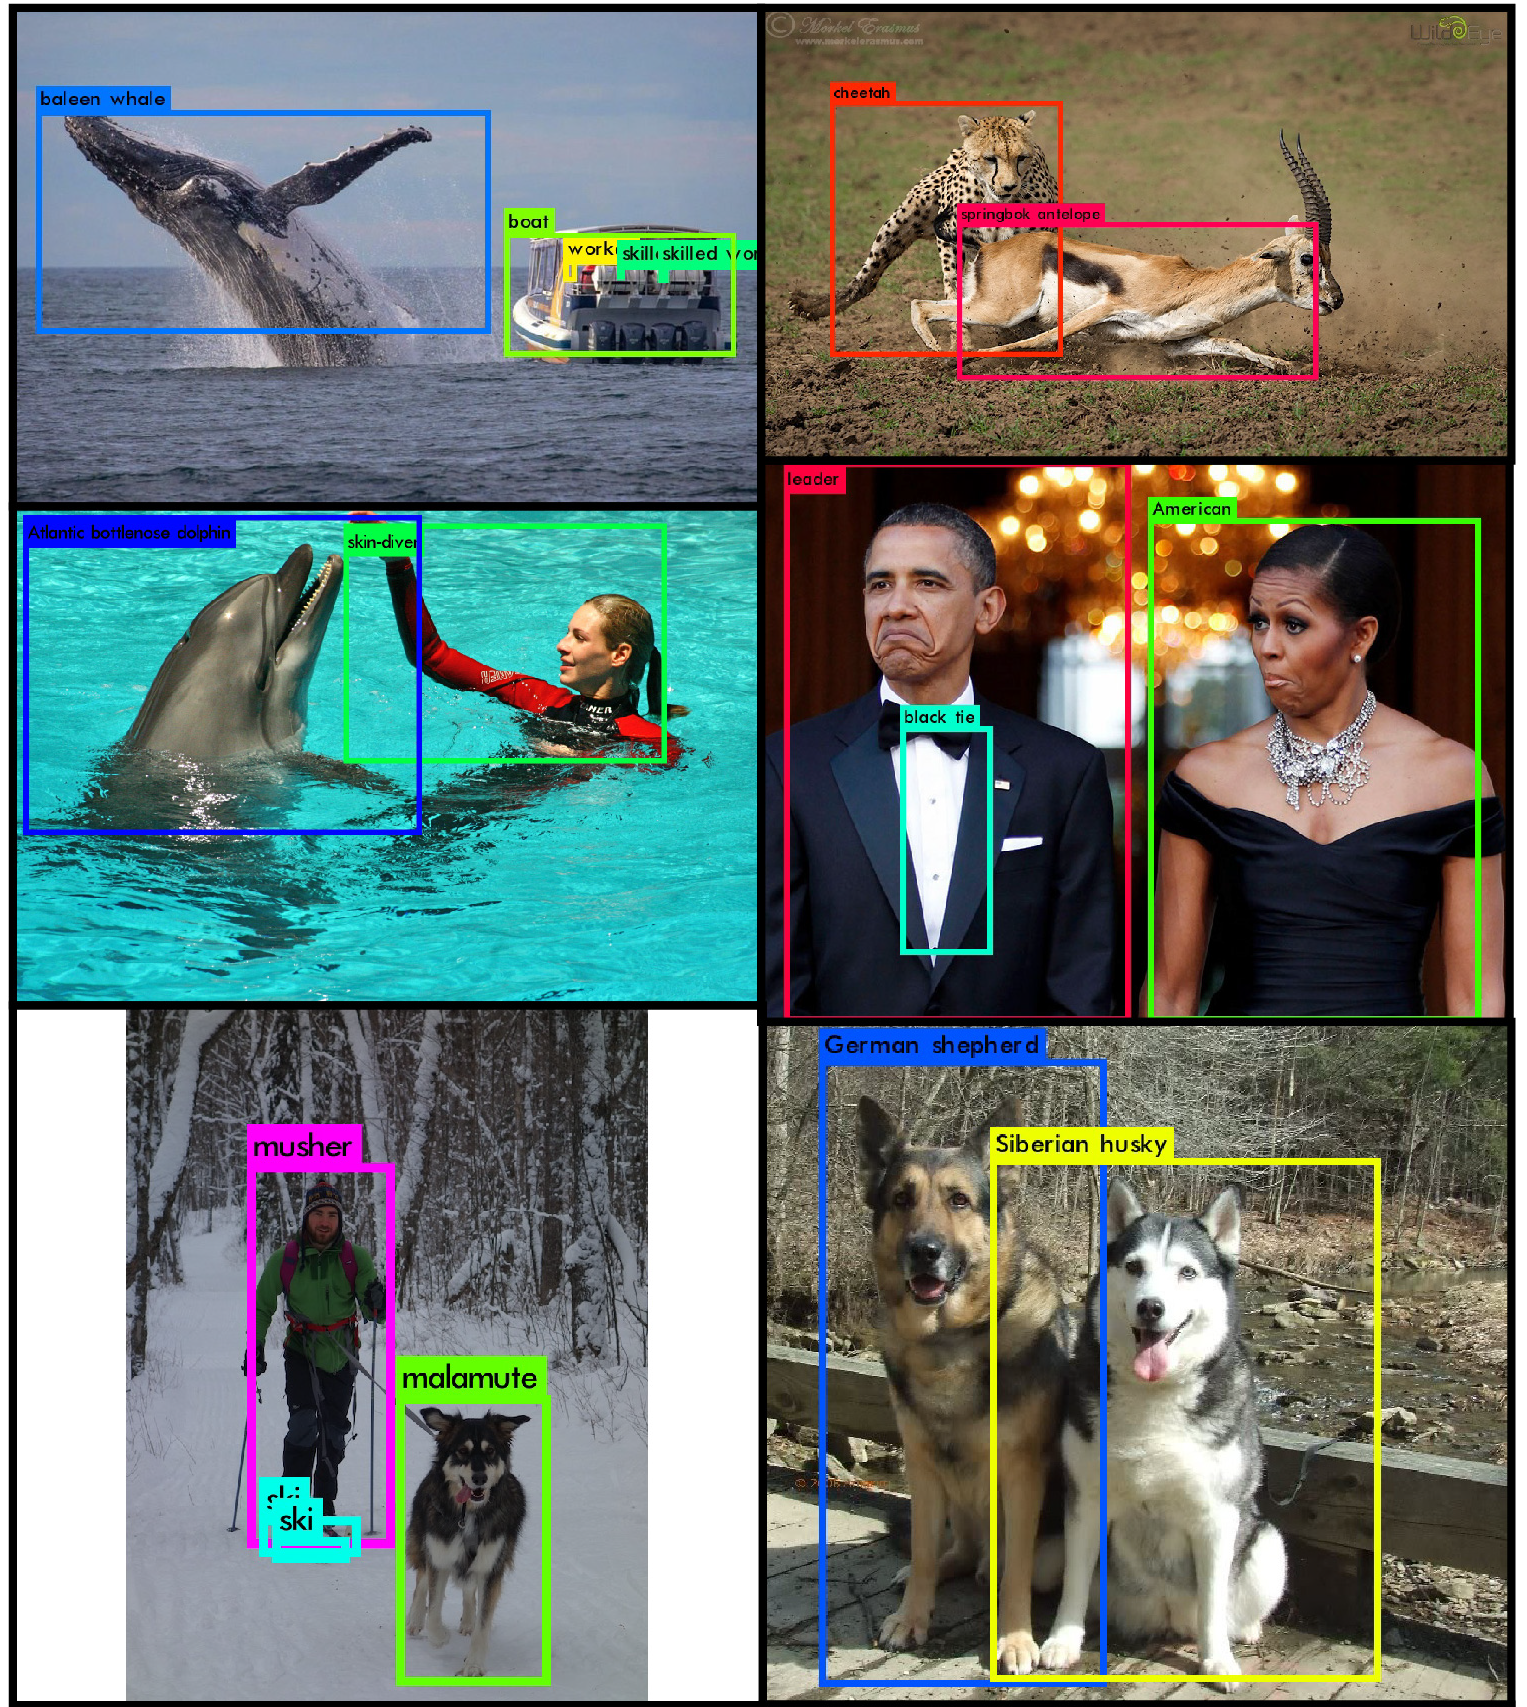
\includegraphics[width=0.7\textwidth]{./back_material_figures/yolo.png}
	\caption[YOLO9000]{Results from YOLO9000, reproduced from \citet{redmon2017}.  The figure shows the results of the CNN when applied to ImageNet data, and its ability to both locate and classify multiple objects in a single image.  }
	\label{fig:disc_yolo}
\end{figure}


\section{Concluding remarks}
\label{sec:disc_conclusions}




\printbibliography[heading=subbibliography]
\end{refsection}
\cleardoublepage

\cleardoublepage % dump remaining floats before end of chapter and ensure the next chapter starts on odd (right-hand) side
\fancyhead[RE]{\leftmark}
\fancyhead[LO]{\rightmark}


\onehalfspacing
\chapter*{Appendix A: Supporting information for Chapter \ref{ch:publication1}}


\noindent\textbf{Contents of this file}
\begin{enumerate}
\item Text S1 to S3
\item Figures S1 to S2
\end{enumerate}



\noindent\textbf{Introduction}
From a paper....

\cleardoublepage % dump remaining floats before end of chapter and ensure the next chapter starts on odd (right-hand) side
\fancyhead[RE,LO]{Appendix A}
\fancyhead[RO,LE]{\thepage}



\end{document}
